% TODO

A fin de probar el algoritmo propuesto, decidimos probarlo realizando la conversión del modelo \textit{Teacup} de algún modelo adicional, elegimos para ello el modelo epidemiológico \textit{SIR}.

Como puede verse en esta la figura \ref{fig:SIR_sd} este modelo cuenta de tres \textbf{stocks}, \textit{Suceptible}, \textit{Infected}, \textit{Recovered}, unidos mediante dos \textbf{flows}, de  \textit{Succumbing} y \textit{Recovering}. Las constantes auxiliares en este modelo son la población total (\textit{Total Population}), tasa de transmisión (\textit{Contact Infectivity}) y duración (\textit{Duration}). En violeta se muestran la información de los \textbf{stocks} que requieren los flujos para sus calculos.

En la figura \ref{fig:SIR_devs_flattened} muestra el modelo \texttt{DEVS} equivalente. En color azul los atómicos \textit{Fplus} y \textit{Fminus} asociados al flujo \textit{Succumbing}, mientras que en naranja se observan los atómicos \textit{Fplus} y \textit{Fminus} asociados al flujo \textit{Recovering}. 

También puede verse en violeta  las conexiones que requieren los atómicos que representan los flujos de los integradores (que son producto de la traducción de los stocks), ya que utilizan estos valores para sus cálculos, tal como se observaba en el modelo original en \textit{System Dynamics} (figura \ref{fig:SIR_sd}). 

En rojo pueden verse los atómicos de los flujos que no son utilizados en el modelo, pero que igualmente dejamos por completitud, a fin de dejar explícito que esos atómicos podrían estar si hubiera un \textbf{inflow} o \textbf{outflow} que se les corresponda.

Como ya explicamos anteriormente, por simplicidad el algoritmo sólo generará la versión aplanada del modelo \texttt{DEVS}, aunque generamos el esquema del modelo con acoplados que puede verse en la figura \ref{fig:SIR_devs}.


\begin{figure}[!h]
\centering
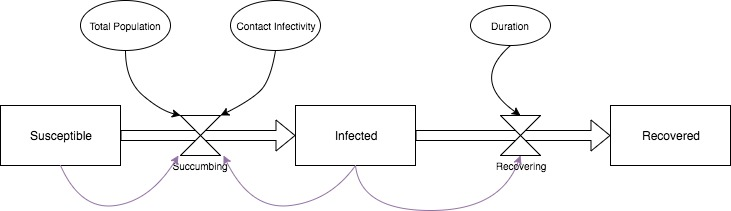
\includegraphics[scale=0.5]{imagenes/SIR_sd.jpg}
\caption{Modelo SIR expresado en System Dynamics en formato gráfico}
\label{fig:SIR_sd}
\end{figure}
\begin{figure}[!h]
\centering
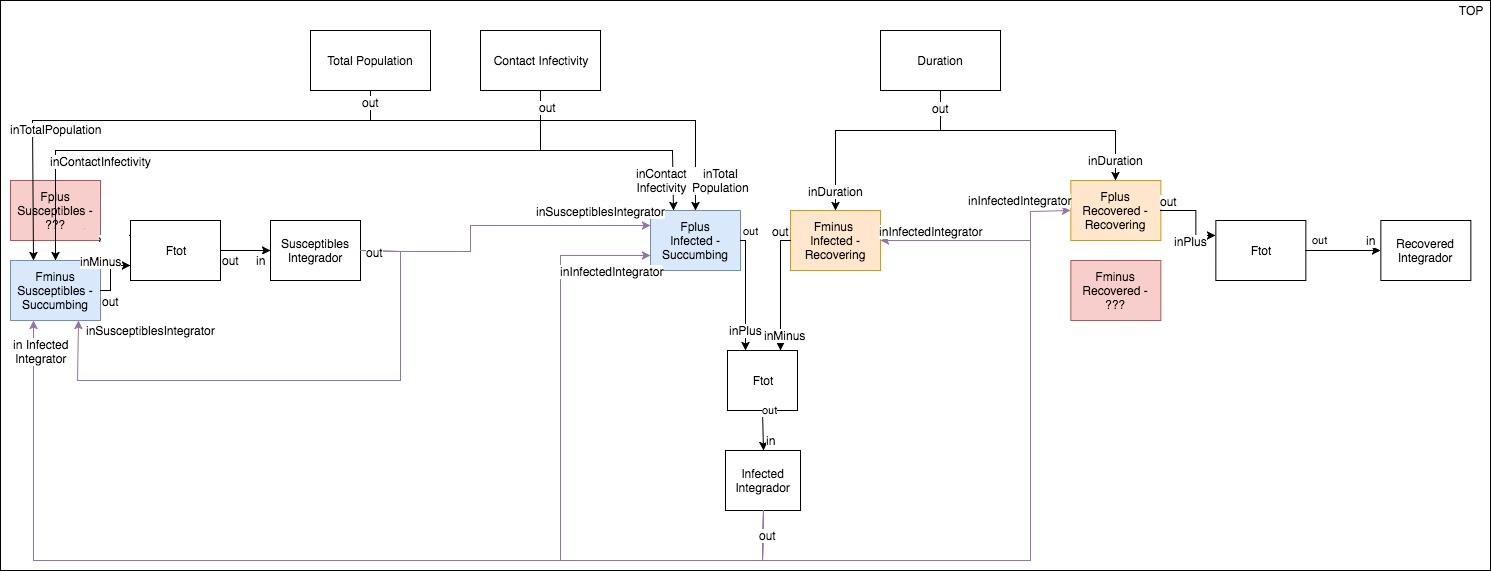
\includegraphics[scale=0.3]{imagenes/SIR_devs_flattened.jpg}
\caption{Modelo SIR expresado en DEVS en formato gráfico}
\label{fig:SIR_devs_flattened}
\end{figure}
\begin{figure}[!h]
\centering
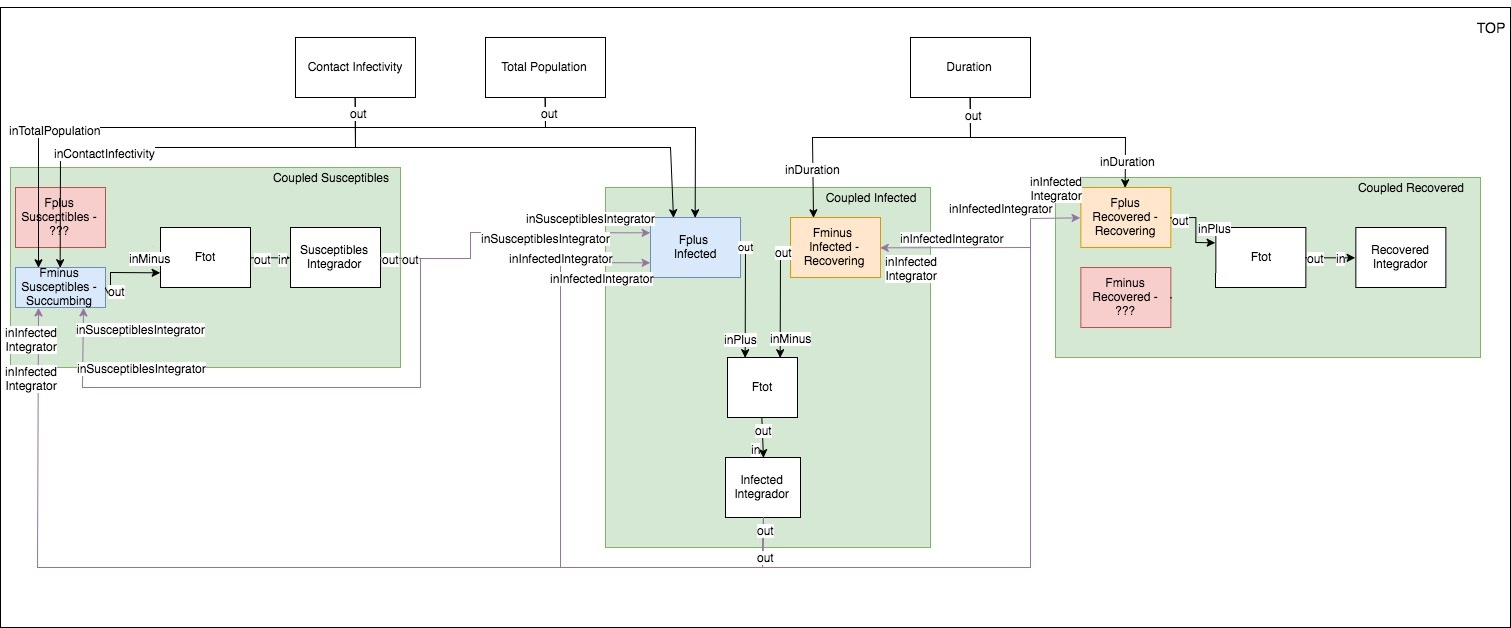
\includegraphics[scale=0.3]{imagenes/SIR_devs.jpg}
\caption{Modelo SIR expresado en DEVS en formato gráfico con varios niveles de acoplamiento}
\label{fig:SIR_devs}
\end{figure}
% TODO

\subsubsection{Generación de modelo ejecutable en CD++}
